\section{MTDA+N Framework} \label{sec:mtda+n}
Ralph and Monu (2014) \cite{Ralph2014} base their article on the MDA framework (Section \ref{sec:mda}) and the elemental tetrad (Section \ref{sec:elemental-tetrad}).
They recognize both frameworks as useful tools for reasoning about game design and being commonly cited in research.
Nonetheless, relying on two separate works is inefficient as they share redundancy.
Integrating these frameworks serves the purpose of working towards a unified game theory covering all relevant areas adequately.
Mechanics and aesthetics are present in either model and the authors generally describe similar ideas.
Technology from Schell's elemental tetrad \cite{Schell2014} and dynamics MDA by Hunicke et al. \cite{Hunicke2004} are also transferred into the integrated framework.

\subsection{Narrative}
According to the authors of MTDA+N the term story carries too much overloaded meaning and is not necessarily suitable for many games lacking traditional stories (e.g. Tetris).
Instead they propose the term narrative which is categorized into three distinctive types.
They will be discussed in the following sections.

\subsubsection{Embedded Narrative}
An embedded narrative is actual content of the game itself.
It is told by the game designers through in-game mechanisms like cutscenes, audio dialogue or graphic artwork.
This fits very well with the string of pearls method discussed by \citeauthor{Schell2014} (Section \ref{sec:story-methods}).
The embedded narrative would take place in between the pearls along the string.

\subsubsection{Emergent Narrative}
In contrast to the embedded narratives the \textit{emergent} variant is only created when players actually use the game.
The name already suggests that the narrative emerges as players take part in the game world.
Certain actions can trigger a chain of events which in turn created sequences of interesting events.
Games acting as story machines (Section \ref{sec:story-methods}) are essentially producing emergent narratives governed by the behavior of players.
Players are effectively responsible for emergent narratives and stories are dependant on how they perceive events in the game.

\subsubsection{Interpreted Narrative}
Players are constantly interpreting both embedded and emergent narratives.
This interpretation is not part of the game itself but rather resides in the mental representation in a player's mind \cite{Ralph2014}.
Therefore, the interpreted narrative acts on the level of aesthetics and influences the experience of a game.

\subsection{Model}
Finally, merging the MDA framework (Figure \ref{fig:mda}) and elemental tetrad (Figure \ref{fig:elemental-tetrad}) results in the \textit{Mechanics, Technology, Dynamics, Aesthetics plus Narratives} framework (MTDA+N) depicted in Figure \ref{fig:mtda+n}.

\begin{figure}[H]
    \centering
    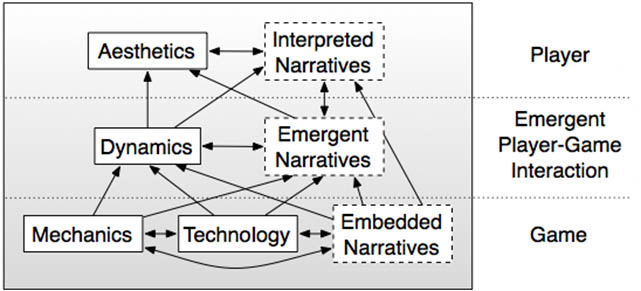
\includegraphics[width=8cm]{assets/mtda+n.jpg}
    \caption{MTDA+N framework\protect\footnotemark}
    \label{fig:mtda+n}
\end{figure}
\footnotetext{\url{http://www.firstpersonscholar.com/a-working-theory-of-game-design}, Accessed: 02-03-2018}

Player primarily interact with mechanics and experience the embedded narrative.
These interactions result in behavioral dynamics of the game and potentially unravels emergent narratives.
Finally, aesthetics and the interpreted narrative reside in the player's mental state and essentially form the experience.